\documentclass[tikz, border=3mm]{standalone}
\usepackage{tikz}
\usetikzlibrary{arrows.meta, positioning}

\begin{document}
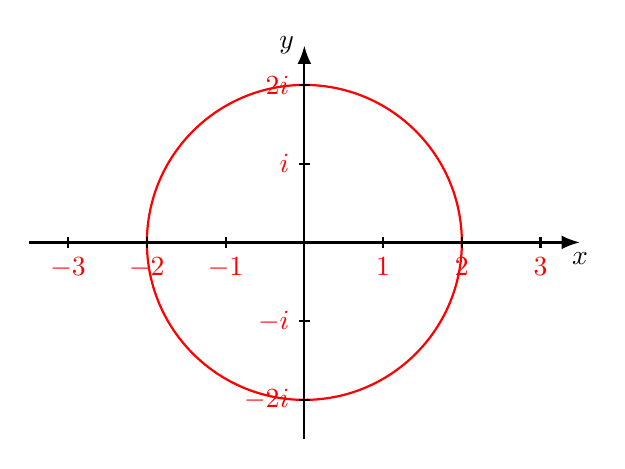
\begin{tikzpicture}[
    >=Latex, % Set defau	lt arrow tip style
    axis/.style={->, thick}, % Style for axes
    pathstyle/.style={red, thick}, % Style for the circle path
    labelstyle/.style={red}, % Style for labels
    tick/.style={thick} % Style for tick marks
]

    % Define radius
    \def\radius{2}

    % Axes (adjust limits to include ticks)
    \draw[axis] (-3.5, 0) -- (3.5, 0) node[below] {$x$};
    \draw[axis] (0, -2.5) -- (0, 2.5) node[left] {$y$};

    % Draw the red circle
    \draw[pathstyle] (0,0) circle (\radius);

    % Ticks and Labels on x-axis
    \foreach \x in {-3, -2, -1, 1, 2, 3} {
        \draw[tick] (\x, -2pt) -- (\x, 2pt);
        \node[labelstyle, below=2pt] at (\x, 0) {$\x$};
    }

    % Ticks and Labels on y-axis
    % Use \ylab to store the label text
    \foreach \y/\ylab in {-2/{-2i}, -1/{-i}, 1/{i}, 2/{2i}} {
        \draw[tick] (-2pt, \y) -- (2pt, \y);
        \node[labelstyle, left=2pt] at (0, \y) {$\ylab$};
    }

\end{tikzpicture}
\end{document}